%!TEX root = 00_main.tex
% ============================================================================
% ADVANCED SLIDES - DIAGRAMS, EMBEDS, AND SPECIAL FEATURES
% ============================================================================

\section{Diagrams and Drawings}

% --- TikZ Flowchart ---
\begin{frame}{Process Flowchart (TikZ)}
    \centering
    \begin{tikzpicture}[node distance=1.5cm, auto,
        block/.style={rectangle, draw, fill=mainblue!20, text width=2.5cm, text centered, rounded corners, minimum height=1cm},
        arrow/.style={->, >=stealth, thick}]

        \node[block] (input) {Wind Data};
        \node[block, right of=input, xshift=2cm] (process) {Aeroelastic Model};
        \node[block, right of=process, xshift=2cm] (output) {Load Time Series};
        \node[block, below of=process] (fatigue) {Fatigue Analysis};

        \draw[arrow] (input) -- (process);
        \draw[arrow] (process) -- (output);
        \draw[arrow] (output) |- (fatigue);
        \draw[arrow] (fatigue) -| (input);
    \end{tikzpicture}

    \vspace{0.5cm}
    {\small Simulation workflow for wind turbine design certification.}
\end{frame}

% --- TikZ Plot ---
\begin{frame}{Data Plot (TikZ)}
    \centering
    \begin{tikzpicture}[scale=0.8]
        \draw[->] (0,0) -- (8,0) node[right] {Wind Speed (m/s)};
        \draw[->] (0,0) -- (0,5) node[above] {Power (MW)};

        % Grid
        \draw[gray!30] (0,0) grid (7.5,4.5);

        % Power curve
        \draw[mainblue, very thick]
            (0,0) -- (0.5,0) -- (1,0.1) -- (2,0.5) -- (3,1.5) -- (4,3) -- (5,4) -- (6,4) -- (7,4);

        % Labels
        \foreach \x in {0,5,10,15,20,25} {
            \node[below, font=\tiny] at (\x/3.5,0) {\x};
        }
        \foreach \y in {0,1,2,3,4,5} {
            \node[left, font=\tiny] at (0,\y) {\y};
        }

        % Annotations
        \draw[red, dashed] (1,0) -- (1,4.5) node[above, font=\tiny] {Cut-in};
        \draw[red, dashed] (5,0) -- (5,4.5) node[above, font=\tiny] {Rated};
        \draw[red, dashed] (7,0) -- (7,4.5) node[above, font=\tiny] {Cut-out};
    \end{tikzpicture}

    \vspace{0.3cm}
    {\small Typical power curve of a 5 MW wind turbine.}
\end{frame}

% --- TikZ Block Diagram ---
\begin{frame}{Control System Block Diagram}
    \centering
    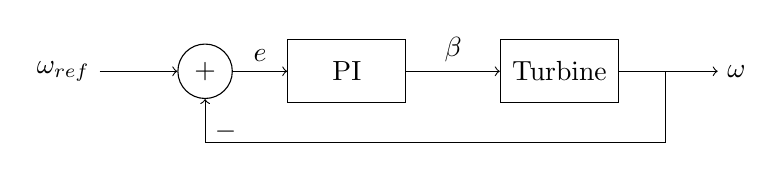
\begin{tikzpicture}[scale=0.9,
        block/.style={rectangle, draw, minimum height=0.8cm, minimum width=1.5cm},
        sum/.style={circle, draw, minimum size=0.5cm}]

        \node[sum] (sum) at (0,0) {$+$};
        \node[block] (controller) at (2,0) {PI};
        \node[block] (plant) at (5,0) {Turbine};
        \node (output) at (7.5,0) {$\omega$};
        \node (input) at (-2,0) {$\omega_{ref}$};

        \draw[->] (input) -- (sum);
        \draw[->] (sum) -- (controller) node[midway, above] {$e$};
        \draw[->] (controller) -- (plant) node[midway, above] {$\beta$};
        \draw[->] (plant) -- (output);
        \draw[->] (6.5,0) -- (6.5,-1) -- (0,-1) -- (sum) node[near start, right] {$-$};
    \end{tikzpicture}

    \vspace{0.5cm}
    {\small Pitch control loop for rotor speed regulation.}
\end{frame}

\section{External Links and Embedded Files}

% --- Links to External Files ---
\begin{frame}{Links to External Files}
    Click links below to open files (must be in same folder as PDF):

    \vspace{0.5cm}

    \begin{itemize}
        \item \href{run:example_figure.png}{Open example\_figure.png} (external link)
        \item \href{run:00_main.tex}{Open source file (00\_main.tex)}
        \item \href{run:01_slides.tex}{Open slides source}
    \end{itemize}

    \vspace{0.5cm}

    Web links:
    \begin{itemize}
        \item \href{https://www.nrel.gov/wind/}{NREL Wind Energy Research}
        \item \href{https://www.iec.ch}{IEC Standards}
    \end{itemize}

    \vspace{0.3cm}
    {\small\textit{Note: External file links work when PDF is in the same folder.}}
\end{frame}

% --- Embedded/Attached Files ---
\begin{frame}[fragile]{Embedded Files in PDF}
    Files can be attached to this PDF using attachfile2 package:

    \vspace{0.3cm}

    \begin{lstlisting}[basicstyle=\ttfamily\small, frame=none, numbers=none]
\textattachfile{data.csv}{Click to open data}
\textattachfile{code.py}{Click to open code}
    \end{lstlisting}

    \vspace{0.3cm}

    {\small Files are embedded inside the PDF and can be extracted by the viewer.}

    \vspace{0.3cm}

    \textit{Useful for sharing data, code, or supplementary materials.}

    \vspace{0.3cm}

    {\footnotesize\textbf{Note:} Uncomment attachfile2 examples when files exist.}
\end{frame}

\section{Beamer Special Features}

% --- Overlays/Animations ---
\begin{frame}{Step-by-Step Reveal (Overlays)}
    Design process phases:

    \begin{enumerate}
        \item<1-> \textbf{Conceptual Design} -- Define requirements
        \item<2-> \textbf{Preliminary Design} -- Initial sizing
        \item<3-> \textbf{Detailed Design} -- FEM analysis
        \item<4-> \textbf{Validation} -- Testing and certification
    \end{enumerate}

    \vspace{0.5cm}

    \only<1>{Start with project requirements and constraints.}
    \only<2>{Perform initial aerodynamic and structural sizing.}
    \only<3>{Run detailed simulations and optimize.}
    \only<4>{Validate against standards (IEC 61400).}
\end{frame}

% --- Blocks ---
\begin{frame}{Information Blocks}
    \begin{block}{Definition}
        The \textbf{capacity factor} is the ratio of actual energy produced to the maximum possible energy output over a period.
    \end{block}

    \begin{exampleblock}{Example}
        A 5 MW turbine producing 15,000 MWh/year has a capacity factor of:
        $CF = \frac{15000}{5 \times 8760} = 34.2\%$
    \end{exampleblock}

    \begin{alertblock}{Warning}
        Capacity factor varies significantly with site conditions and turbine selection.
    \end{alertblock}
\end{frame}

% --- Table Example ---
\begin{frame}{Data Table}
    \centering
    \begin{tabular}{lrrr}
        \toprule
        \textbf{Parameter} & \textbf{IEA 15 MW} & \textbf{DTU 10 MW} & \textbf{NREL 5 MW} \\
        \midrule
        Rated Power (MW)    & 15.0  & 10.0  & 5.0   \\
        Rotor Diameter (m)  & 240   & 178   & 126   \\
        Hub Height (m)      & 150   & 119   & 90    \\
        Tip Speed (m/s)     & 95    & 90    & 80    \\
        \bottomrule
    \end{tabular}

    \vspace{0.5cm}
    {\small Reference wind turbine specifications for research.}
\end{frame}

% --- Multi-column with Pause ---
\begin{frame}{Comparison Layout}
    \begin{columns}[T]
        \begin{column}{0.48\textwidth}
            \textbf{Onshore Wind}
            \begin{itemize}
                \item Lower installation cost
                \item Easier maintenance access
                \item Visual/noise concerns
                \item Limited to smaller turbines
            \end{itemize}
        \end{column}
        \begin{column}{0.48\textwidth}
            \textbf{Offshore Wind}
            \begin{itemize}
                \item Higher wind speeds
                \item Larger turbines possible
                \item Higher CAPEX/OPEX
                \item Complex logistics
            \end{itemize}
        \end{column}
    \end{columns}
\end{frame}
